\documentclass[10pt]{article}
\usepackage{float}
\usepackage{amsmath}
\usepackage{paralist}
\usepackage{setspace}
\usepackage{listings}
\usepackage{graphicx}
\usepackage[english]{babel}
\usepackage{geometry}
\usepackage{subcaption}
\usepackage[utf8]{inputenc}
\usepackage{listings}
\usepackage{color}
\usepackage{subcaption}
\usepackage{hyperref}
\usepackage{mathtools}

\newcommand\floor[1]{\lfloor#1\rfloor}
\newcommand\ceil[1]{\lceil#1\rceil}

\begin{document}


\definecolor{mygreen}{rgb}{0,0.6,0}
\definecolor{mygray}{rgb}{0.5,0.5,0.5}
\definecolor{mymauve}{rgb}{0.58,0,0.82}

\lstset{ %
  backgroundcolor=\color{white},   % choose the background color; you must add \usepackage{color} or \usepackage{xcolor}
  basicstyle=\footnotesize,        % the size of the fonts that are used for the code
  breakatwhitespace=false,         % sets if automatic breaks should only happen at whitespace
  breaklines=true,                 % sets automatic line breaking
  captionpos=b,                    % sets the caption-position to bottom
  commentstyle=\color{mygreen},    % comment style
  deletekeywords={...},            % if you want to delete keywords from the given language
  escapeinside={\%*}{*)},          % if you want to add LaTeX within your code
  extendedchars=true,              % lets you use non-ASCII characters; for 8-bits encodings only, does not work with UTF-8
  frame=tb,	                   % adds a frame around the code
  keepspaces=true,                 % keeps spaces in text, useful for keeping indentation of code (possibly needs columns=flexible)
  keywordstyle=\color{blue},       % keyword style
  language=Octave,                 % the language of the code
  otherkeywords={*,...},           % if you want to add more keywords to the set
  numbers=left,                    % where to put the line-numbers; possible values are (none, left, right)
  numbersep=5pt,                   % how far the line-numbers are from the code
  numberstyle=\tiny\color{mygray}, % the style that is used for the line-numbers
  rulecolor=\color{black},         % if not set, the frame-color may be changed on line-breaks within not-black text (e.g. comments (green here))
  showspaces=false,                % show spaces everywhere adding particular underscores; it overrides 'showstringspaces'
  showstringspaces=false,          % underline spaces within strings only
  showtabs=false,                  % show tabs within strings adding particular underscores
  stepnumber=2,                    % the step between two line-numbers. If it's 1, each line will be numbered
  stringstyle=\color{mymauve},     % string literal style
  tabsize=2,	                   % sets default tabsize to 2 spaces
  title=\lstname                   % show the filename of files included with \lstinputlisting; also try caption instead of title
}



\onehalfspacing
\begin{titlepage}
\begin{center}
% Oberer Teil der Titelseite:


\textsc{\LARGE University Oldenburg}\\[1.5cm]

\textsc{\Large Wind Physics Measurement Project}\\[0.5cm]


% Title
\newcommand{\HRule}{\rule{\linewidth}{0.5mm}}
\HRule \\[0.4cm]
{ \huge \bfseries Exercise 1 - Handling and preprocessing of measurement data}\\[0.4cm]

\HRule \\[1.5cm]

% Author and supervisor
\begin{minipage}{0.4\textwidth}
\begin{flushleft} \large
\emph{Author:}\\
Jan \textsc{K\"amper}\\
Florian \textsc{B\"orgel}
\end{flushleft}
\end{minipage}
\hfill
\begin{minipage}{0.4\textwidth}
\begin{flushright} \large
\emph{Supervisor:} \\
Matthias \textsc{Wächter}
\end{flushright}
\end{minipage}
\\[3cm]
\vfill



% Unterer Teil der Seite
{\large \today}

\end{center}

\end{titlepage}
\tableofcontents
\newpage
\section*{Introduction}
In this third learning unit of the Wind Physics Measurement Project the goal was to perform a long term assessment of wind resources for the windpark Kriegers Flak2 close to the FINO2 met mast in the Baltic Sea. As reanalysis data for wind speeds and directions a 24 year time-series MERRA-2 was provided. This report describes how the short-term measurement data and the reanalysis data were taken to derive long-term corrected data for FINO2 by applying the Sectoral Regression MCP method.
 
\section{Task 1: Synchronizing the data}
In task 1 we were asked to synchronize the data of FINO2 and MERRA-2. The data of FINO2 was provided in 10 minute-averages over five years starting in January 2010. The MERRA-2 data is the so called long-term data provided in one hour-averages, ranging from 1992 to 2016.
Preprocessing of the data included neglecting all measured data of FINO2 after the end of May 2014 and computation of one hour averages at a height of $92m$.
Since we only synchronize overlapping time intervals of FINO2 and MERRA-2 we had to look up the according time stamps in both given time formats: 
\begin{lstlisting}
timestamps = raw_data.Var1(:,1);
first_timestamp = find(strcmp(timestamps(:), '01.01.2010 00:00'));
last_timestamp = find(strcmp(timestamps(:), '31.05.2014 23:00'));
last_timestampFino2 = find(Fino2.time==datenum('31-May-2014 23:55:00'));
\end{lstlisting}
We used the following routine for converting the 10-minute averages of speed and direction into 1-hour averages:
\begin{lstlisting}
fino2_1h_92 = [];
for i = 1:last_timestampFino2/6
    fino2_1h_92(i,1) = datenum('01-Jan-2010 00:00:00')+(i-1)*1/24;
    range_array_v = fino2_v92((i-1)*6+1:i*6,1);
    range_array_dir = fino2_d91((i-1)*6+1:i*6,1);
    fino2_1h_92(i,3) = nanmean(range_array_v);
    fino2_1h_92(i,2) = nanmean(range_array_dir);
end
\end{lstlisting}
The loop creates a continuous time axis with hour intervals  In addition it calculates the mean of six 10-minutes intervals for wind speeds and wind directions.\\

After preparing the right time intervals we were able to save the data into a variable called connected\_data holding the synchronized data. \\
Synchronizing the data means that we only take into account time stamps for which both measurement systems have valid entries. Incorrect data of FINO2 appears as NaN values. The data of MERRA-2 has additional status columns. $0$ as an entry indicates a correct measurement. Thus we made sure that only those rows are taken into further consideration where both FINO2 and MERRA-2 have valid data. Otherwise rows are omitted by setting them to $NaN$:
\begin{lstlisting}
for i = 1:length(connected_data(:,1))
    if raw_data.Var8(i) ~= 0 || raw_data.Var9(i) ~= 0 || isnan(connected_data(i,2)) == 1 || isnan(connected_data(i,3)) == 1
        connected_data(i,2:5) = NaN;
    end
end
\end{lstlisting}
\section{Task 2: Sorting into 12 wind sectors}
In order to sort the synchronized data into 12 sectors we decided to store the data of different wind sectors in a cell variable. This ways all entries for a certain sector can be easily accessed via an index which can be computed with the simple formula:
\begin{equation*}
 sector = \floor{\frac{direction \cdot 12}{360}}+1 
\end{equation*}
Here is how the wind speeds are sorted according to the directions using this formula:
\begin{lstlisting}
for i = 1:length(connected_data(:,1))
    if ~isnan(connected_data(i,3)) && ~isnan(connected_data(i,4)) && ~isnan(connected_data(i,2))
        sortIndex = floor(connected_data(i,3)/360*12)+1;
        sortedCell{sortIndex*3-2} = [sortedCell{sortIndex*3-2}, connected_data(i,1)]; %timestamp
        sortedCell{sortIndex*3-1} = [sortedCell{sortIndex*3-1}, connected_data(i,4)]; %merra 2
        sortedCell{sortIndex*3} = [sortedCell{sortIndex*3}, connected_data(i,2)]; %fino 2
        sortedCell{37} = [sortedCell{37}, connected_data(i,1)]; %timestamp
        sortedCell{38} = [sortedCell{38}, connected_data(i,4)]; %merra 2
        sortedCell{39} = [sortedCell{39}, connected_data(i,2)]; %fino 2
    end;
end;
\end{lstlisting} 
The variable $sortedCell$ contains 3 vectors for every sector, one for the timestamps and one for the speed at FINO2 and MERRA-2. Additionally the last 3 vectors contain the corresponding values for all data independent of the sector.
The first sector here is from $0^{\circ}-30^{\circ}$. Of course one could as well start with a true north sector of $345^{\circ}-15^{\circ}$ but this a question of definitions.

\section{Task 3: Monthly averages of sectors}
The next step consisted in computing the sector-wise and 1-month averages of the synchronized data. The relevant period consists of 53 months and we have 26 averages to compute, i.e. the MERRA-2 averages and the FINO2 averages for each of the 12 sectors and for the entire data. Hence we obtain a $53 x 27$ matrix where the first column is reserved for an identifier of the month. The variable $avgSectorPerMonth$ holds these averages. In the following code extract it can be seen how the sector-wise data is taken from the $sortedCell$ structure and then filtered by the corresponding month using the $addtodate$ command:
\begin{lstlisting}
for sectorIndex = 1:12
    for monthIndex = 1:53
        valuesInMonthAndSectorMerra2 = sortedCell{sectorIndex*3-1}(find((sortedCell{sectorIndex*3-2} > addtodate(firstMonth,monthIndex-1,'month')) ...
            & (sortedCell{sectorIndex*3-2} <= addtodate(firstMonth,monthIndex,'month'))));
       valuesInMonthAndSectorFino2 = sortedCell{sectorIndex*3}(find((sortedCell{sectorIndex*3-2} > addtodate(firstMonth,monthIndex-1,'month')) ...
            & (sortedCell{sectorIndex*3-2} <= addtodate(firstMonth,monthIndex,'month'))));
        avgSectorPerMonth(monthIndex,sectorIndex*2+2)= nanmean(valuesInMonthAndSectorMerra2);
        avgSectorPerMonth(monthIndex,sectorIndex*2+3)= nanmean(valuesInMonthAndSectorFino2);
    end;
end;
\end{lstlisting} 

\section{Task 4-5: Regressions parameters and plots} 
With all the synchronization and preparation of the data done, we can now start with the analysis. As a first step a regression between FINO2 and MERRA-2 monthly averages will be carried out and linear relationships derived for each sector and for the entire data. The routines $regression()$ and $plotregression()$ are well suited for this purpose where the first supplies the regression parameters $R, m$ and $b$ and the latter graphically illustrates the found relationship. 

\begin{lstlisting}
    [regressionParameters(i,2),  regressionParameters(i,3), regressionParameters(i,4)] = ... 
        regression(avgSectorPerMonth(:,i*2), avgSectorPerMonth(:,i*2+1), 'one');
    regressionParameters(i,1) = regressionParameters(i,2) * regressionParameters(i,2);
    plotregression(avgSectorPerMonth(:,i*2), avgSectorPerMonth(:,i*2+1), 'Regression');
\end{lstlisting}
Figure~\ref{fig:Regression} shows the resulting plots for all 12 sectors and at last for the entire data. 
We can see that a linear relationship models the two datasets quite well. The regression lines for all sectors start with a small vertical offset although there are differences between the various sectors. Regarding the correlation we can see that all sectors except one have a value of $R^2 \geq 0.8$ which was given as quality criteria in the lecture, sector $120^{\circ}-150^{\circ}$ with $R^2=0.75$ being the exception. The majority of the line slopes are slightly larger than $1$, except for sectors $150^{\circ}-180^{\circ}$ and $120^{\circ}-150^{\circ}$.

An overview of all regression parameters is given in the following table~\ref{tab:regParam}.

\begin{figure}[H]
\begin{tabular}{c||c|c|c|c|c|c|c|c}

	& ALL:  $0^{\circ}-360^{\circ}$ &  $0^{\circ}-30^{\circ}$ & $30^{\circ}-60^{\circ}$ & $60^{\circ}-90^{\circ}$ & $90^{\circ}-120^{\circ}$ & $120^{\circ}-150^{\circ}$ & $150^{\circ}-180^{\circ}$ \\
	\hline \hline
    R & 0.9574 &   0.9096 &   0.9391  &  0.9138  &  0.9002  &  0.8681  &  0.9367  &  \\
    \hline
    m & 1.0211 &   0.6329 &   1.0882  &  1.2793  &  1.0177  &  0.8368  &  0.9616  &   \\
    \hline
    b & 1.1831 &   0.8299 &   0.4746  & -0.4634  &  1.3246  &  2.4300  &  0.9867  &  \\

\end{tabular}

\vspace{30 pt}

\begin{tabular}{c||c|c|c|c|c|c|c}

	& $180^{\circ}-210^{\circ}$ & $210^{\circ}-240^{\circ}$ & $240^{\circ}-270^{\circ}$ & $270^{\circ}-300^{\circ}$ & $300^{\circ}-330^{\circ}$ & $330^{\circ}-360^{\circ}$ \\
	\hline \hline
    R   &  0.9311  &  0.9646  &  0.9824  &  0.9768  &  0.9554  &  0.9054 & \\
    \hline
    m &  1.1074  &  1.1520  &  1.1237 &   1.0506 &   1.1058  &  1.0034 & \\
    \hline
    b   &  0.1886  &  0.3036  &  0.2504 &   0.7260  &  0.4979  &  1.0759& \\

\end{tabular}
\caption{Regression parameters for all data and sector-wise}
\label{tab:regParam}
\end{figure}


\begin{figure}[H]
\begin{subfigure}{0.33\textwidth}
  \centering
  \includegraphics[width=1\linewidth]{../figures/scatterPlot_Sector0.jpg}
\end{subfigure}
\begin{subfigure}{0.33\textwidth}
  \centering
  \includegraphics[width=1\linewidth]{../figures/scatterPlot_Sector30.jpg}
\end{subfigure}
\begin{subfigure}{0.33\textwidth}
  \centering
  \includegraphics[width=1\linewidth]{../figures/scatterPlot_Sector60.jpg}
\end{subfigure}
\begin{subfigure}{0.3\textwidth}
  \centering
  \includegraphics[width=1\linewidth]{../figures/scatterPlot_Sector90.jpg}
\end{subfigure}
\begin{subfigure}{0.3\textwidth}
  \centering
  \includegraphics[width=1\linewidth]{../figures/scatterPlot_Sector120.jpg}
\end{subfigure}
\begin{subfigure}{0.3\textwidth}
  \centering
  \includegraphics[width=1\linewidth]{../figures/scatterPlot_Sector150.jpg}
\end{subfigure}
\begin{subfigure}{0.3\textwidth}
  \centering
  \includegraphics[width=1\linewidth]{../figures/scatterPlot_Sector180.jpg}
\end{subfigure}
\begin{subfigure}{0.3\textwidth}
  \centering
  \includegraphics[width=1\linewidth]{../figures/scatterPlot_Sector210.jpg}
\end{subfigure}
\begin{subfigure}{0.3\textwidth}
  \centering
  \includegraphics[width=1\linewidth]{../figures/scatterPlot_Sector240.jpg}
\end{subfigure}
\begin{subfigure}{0.3\textwidth}
  \centering
  \includegraphics[width=1\linewidth]{../figures/scatterPlot_Sector270.jpg}
\end{subfigure}
\begin{subfigure}{0.3\textwidth}
  \centering
  \includegraphics[width=1\linewidth]{../figures/scatterPlot_Sector300.jpg}
\end{subfigure}
\begin{subfigure}{0.3\textwidth}
  \centering
  \includegraphics[width=1\linewidth]{../figures/scatterPlot_Sector330.jpg}
\end{subfigure}
\begin{subfigure}{0.3\textwidth}
  \centering
  \includegraphics[width=1\linewidth]{../figures/scatterPlot_AllSectors.jpg}
\end{subfigure}
  \caption{Regressions Plots}
\label{fig:Regression}
\end{figure}



\section{Task 6: Deriving long-term predicted data}
With the previous tasks the measurement and correlation of the data has been successfully carried out. We now proceed to the last step of the MCP method which is prediction. The found relationships from the linear regression enable deriving long-term predicted data, i.e. the FINO2 data is extrapolated to the 24 years period. The data structures set up in the previous tasks make it easy to efficiently apply the relationships for each sector with only 4 lines of code:
\begin{lstlisting}
for i = 1:length(raw_data.Var2(:))
    sectorIndex= floor(raw_data.Var3(i) /360*12)+1;
    longTermCorrectedFino2(i,1) = raw_data.Var2(i) * regressionParameters(sectorIndex,2) + regressionParameters(sectorIndex,3);
    longTermCorrectedFino2(i,2) = raw_data.Var3(i);
end;
\end{lstlisting} 
Again a sector index is calculated from the direction of the MERRA-2 data row and then the found regression parameters $m$ and $b$ are used to derive the long-term corrected FINO2 data from 1992-2016 in 1 hour time-intervals. The wind directions are copied 1-to-1 from the MERRA-2 data.

\section{Task 7-8: Calculating Weibull parameters for the long-term predicted data and plot}
We now take a closer look at the distribution of the sector-wise wind speeds for the long-term predicted data. The routine $wblfit()$ combined with our data set up in the previous task complete this task efficiently:
\begin{lstlisting}
for sectorIndex=1:12
    weibullParam(sectorIndex+1,:) = wblfit(longTermCorrectedFino2(find(longTermCorrectedFino2(:,2) >= (sectorIndex-1)*30 & ... 
        longTermCorrectedFino2(:,2) < sectorIndex*30),1));
end;
\end{lstlisting} 

With the Weibull parameters calculated for each sector and also for the entire data we can then put the Weibull curves into one single plot in order to detect differences for the 12 sectors, see Figure~\ref{fig:weibullPlots}. We state that the distributions are considerably different. E.g. sectors 3 and 6 have quite low Weibull scale parameters, around $A \approx 7.8$, which leads to the corresponding curves being shifted to the left with lower mean wind speeds. On the opposite side sectors 9 and 10 have larger scale parameters of around $A \approx 11.5$ accounting for a higher mean and the curves lying on the right side of the spectrum. Not surprisingly the Weibull distribution of the entire data is pretty much in the middle of the sector-wise distribution curves. Differences of the various sectors can be explained with obstacles which influence the wind speed depending on the specific direction.
\begin{figure}
\centering
  \includegraphics[width=0.7\linewidth]{../figures/weibullPlots.jpg}
  \caption{Weibull curves sector-wise}
  \label{fig:weibullPlots}
\end{figure}


\section{Task 9: Comparing short-term measured and long-term predicted data sector-wise}
After comparison of the sector-wise Weibull distributions next a comparison of the short-term measured and long-term predicted data for FINO2 will be carried out. The Weibull parameters of the long-term predicted data have already been computed in the previous task. It remains to obtain the corresponding values for short-term. 
\begin{lstlisting}
    weibullParam_shortTerm(sectorIndex,:) = wblfit(sortedCell{(sectorIndex-1)*3});
\end{lstlisting} 

\begin{figure}[H]
\begin{subfigure}{0.3\textwidth}
  \centering
  \includegraphics[width=1\linewidth]{../figures/shortVsLongTerm_Sector0.jpg}
\end{subfigure}
\begin{subfigure}{0.3\textwidth}
  \centering
  \includegraphics[width=1\linewidth]{../figures/shortVsLongTerm_Sector30.jpg}
\end{subfigure}
\begin{subfigure}{0.3\textwidth}
  \centering
  \includegraphics[width=1\linewidth]{../figures/shortVsLongTerm_Sector60.jpg}
\end{subfigure}
\begin{subfigure}{0.3\textwidth}
  \centering
  \includegraphics[width=1\linewidth]{../figures/shortVsLongTerm_Sector90.jpg}
\end{subfigure}
\begin{subfigure}{0.3\textwidth}
  \centering
  \includegraphics[width=1\linewidth]{../figures/shortVsLongTerm_Sector120.jpg}
\end{subfigure}
\begin{subfigure}{0.3\textwidth}
  \centering
  \includegraphics[width=1\linewidth]{../figures/shortVsLongTerm_Sector150.jpg}
\end{subfigure}
\begin{subfigure}{0.3\textwidth}
  \centering
  \includegraphics[width=1\linewidth]{../figures/shortVsLongTerm_Sector180.jpg}
\end{subfigure}
\begin{subfigure}{0.3\textwidth}
  \centering
  \includegraphics[width=1\linewidth]{../figures/shortVsLongTerm_Sector210.jpg}
\end{subfigure}
\begin{subfigure}{0.3\textwidth}
  \centering
  \includegraphics[width=1\linewidth]{../figures/shortVsLongTerm_Sector240.jpg}
\end{subfigure}
\begin{subfigure}{0.3\textwidth}
  \centering
  \includegraphics[width=1\linewidth]{../figures/shortVsLongTerm_Sector270.jpg}
\end{subfigure}
\begin{subfigure}{0.3\textwidth}
  \centering
  \includegraphics[width=1\linewidth]{../figures/shortVsLongTerm_Sector300.jpg}
\end{subfigure}
\begin{subfigure}{0.3\textwidth}
  \centering
  \includegraphics[width=1\linewidth]{../figures/shortVsLongTerm_Sector330.jpg}
\end{subfigure}
\begin{subfigure}{0.3\textwidth}
  \centering
  \includegraphics[width=1\linewidth]{../figures/shortVsLongTerm_AllSectors.jpg}
\end{subfigure}
  \caption{Regressions Plots}
\label{fig:CompWeibull}
\end{figure}


The 13 plots (1 for the entire data and 12 for the sectors) are depicted in Figure~\ref{fig:CompWeibull}. The blue curves represent the long-term corrected data while the red curves represent the short-term measured data. In the 13 plots we can clearly see that the Weibull distributions of long and short-term data are strongly correlated. The peaks of the blue and red curve are for all sectors almost vertically aligned. However, in most cases the short-term data Weibull peak lies considerably below the long-term Weibull peak which means that the predicted wind is weaker than the wind actually measured at the met-mast in the short-term period, i.e. the Weibull A parameter is higher for the short-term data. The unusually weak wind period in the 1990s could account for this trend, i.e. the wind is stronger then expected because the reanalyzed data used for prediction origins from a low wind period. This holds for all sectors except sector 1, i.e. $0^{\circ}-30^{\circ}$, where the long-term prediction yields a stronger wind speed than actually measured at FINO2. We assume that the reason for this irregularity is some obstacle which is specific to the FINO2 location, most probably the met-mast itself.

\section{Task 10-11: Regression quality, bias and discussion}
The table in Figure~\ref{fig:overview} shows in its 3 rows: $R^2$ and the two biases $\frac{A_{long}}{A_{short}}$ as well as $\frac{k_{long}}{k_{short}}$ for the entire data (1st column) and the 12 different sectors (columns 2-13). 

\begin{figure}[H]
\centering
  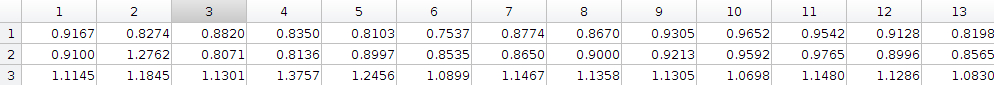
\includegraphics[width=1\linewidth]{../figures/overview.jpg}
  \caption{Overview table of $R^2$ and bias of Weibull parameters}
  \label{fig:overview}
\end{figure}

We state that the further a scaling factor of the Weibull $A$ or $k$ parameter is from $1$ the less precise the prediction of the long-term data becomes. For example see sector 3 where the two Weibull plots in Task 9 are very much different, here we can see the reason for this which is that the scaling factor is only around $0.8$. An opposite example is sector 10 where both $A$ and $k$ parameter have a scaling factor between long and short-term data relatively close to $1$. So in this case prediction does approach the actually measured short-term data better. The same holds for the regression parameter $R^2$. If the regression achieves a higher value here the more correlated and the less uncertain will be the long-term prediction.

\newpage

\appendix
\section{Appendix}
\subsection{Code}
\begin{lstlisting}
%% Task 1
load('WMP_WEnMet_data.mat');
raw_data = readtable('MERRA2_N55.000_E013.125_1992-2016.txt','Delimiter','tab','HeaderLines',26);

fino2_v92 = Fino2.ws92';
fino2_d91 = Fino2.wd91';

%compute indices for relevant timestamps in both formats (Merra2 and Fino2)
timestamps = raw_data.Var1(:,1);
first_timestamp = find(strcmp(timestamps(:), '01.01.2010 00:00'));
last_timestamp = find(strcmp(timestamps(:), '31.05.2014 23:00'));
last_timestampFino2 = find(Fino2.time==datenum('31-May-2014 23:55:00'));

% Check status flags of Merra2 Data
if any(raw_data.Var9(:)) ~= 0
    disp('error');
end

%creating 1h averages for FINO2 over relevant period
fino2_1h_92 = [];
for i = 1:last_timestampFino2/6
    fino2_1h_92(i,1) = datenum('01-Jan-2010 00:00:00')+(i-1)*1/24;
    range_array_v = fino2_v92((i-1)*6+1:i*6,1);
    range_array_dir = fino2_d91((i-1)*6+1:i*6,1);
    fino2_1h_92(i,3) = nanmean(range_array_v);
    fino2_1h_92(i,2) = nanmean(range_array_dir);
end

%connected_data contains 1h averages of merra2 and fino2 data as well as
%corresponding directions and timestamps
connected_data(:,1) = fino2_1h_92(:,1); %timstamps (1h intervals from 01.01.2010 until 31.05.2014)
connected_data(:,2) = fino2_1h_92(:,3); %speed fino 2
connected_data(:,3) = fino2_1h_92(:,2); %direction fino2
connected_data(:,4) = raw_data.Var2(first_timestamp:last_timestamp); %speed merra2
connected_data(:,5) = raw_data.Var3(first_timestamp:last_timestamp); %direction merra2

for i = 1:length(connected_data(:,1))
    if raw_data.Var8(i) ~= 0 || raw_data.Var9(i) ~= 0 || isnan(connected_data(i,2)) == 1 || isnan(connected_data(i,3)) == 1
        connected_data(i,2:5) = NaN;
    end
end


%% Task 2
for i=1:39
    sortedCell{i} = [];
end;

%compute sector index and put the relevant data (merra2 and fino2 speed and
%timestamp) into cell structure by appending
for i = 1:length(connected_data(:,1))
    if ~isnan(connected_data(i,3)) && ~isnan(connected_data(i,4)) && ~isnan(connected_data(i,2))
        sortIndex = floor(connected_data(i,3)/360*12)+1;
        sortedCell{sortIndex*3-2} = [sortedCell{sortIndex*3-2}, connected_data(i,1)]; %timestamp
        sortedCell{sortIndex*3-1} = [sortedCell{sortIndex*3-1}, connected_data(i,4)]; %merra 2
        sortedCell{sortIndex*3} = [sortedCell{sortIndex*3}, connected_data(i,2)]; %fino 2
        sortedCell{37} = [sortedCell{37}, connected_data(i,1)]; %timestamp
        sortedCell{38} = [sortedCell{38}, connected_data(i,4)]; %merra 2
        sortedCell{39} = [sortedCell{39}, connected_data(i,2)]; %fino 2
    end;
end;

%% Task 3
avgSectorPerMonth = zeros(53,27);
firstMonth = datenum('01-Jan-2010');

%first column: month indices
for i=1:53
    avgSectorPerMonth(i,1) = addtodate(firstMonth,i-1,'month');
end;

%second column: monthly averages sector independent
for i=1:53
     valuesInMonthAndSectorMerra2 = sortedCell{38}(find((sortedCell{37} > addtodate(firstMonth,i-1,'month')) ...
            & (sortedCell{37} <= addtodate(firstMonth,i,'month'))));
     valuesInMonthAndSectorFino2 = sortedCell{39}(find((sortedCell{37} > addtodate(firstMonth,i-1,'month')) ...
            & (sortedCell{37} <= addtodate(firstMonth,i,'month'))));
     avgSectorPerMonth(i,2)= nanmean(valuesInMonthAndSectorMerra2);
     avgSectorPerMonth(i,3)= nanmean(valuesInMonthAndSectorFino2);
end;

%%next: wind speeds for both locations as monthly average per sector
for sectorIndex = 1:12
    for monthIndex = 1:53
        valuesInMonthAndSectorMerra2 = sortedCell{sectorIndex*3-1}(find((sortedCell{sectorIndex*3-2} > addtodate(firstMonth,monthIndex-1,'month')) ...
            & (sortedCell{sectorIndex*3-2} <= addtodate(firstMonth,monthIndex,'month'))));
       valuesInMonthAndSectorFino2 = sortedCell{sectorIndex*3}(find((sortedCell{sectorIndex*3-2} > addtodate(firstMonth,monthIndex-1,'month')) ...
            & (sortedCell{sectorIndex*3-2} <= addtodate(firstMonth,monthIndex,'month'))));
        avgSectorPerMonth(monthIndex,sectorIndex*2+2)= nanmean(valuesInMonthAndSectorMerra2);
        avgSectorPerMonth(monthIndex,sectorIndex*2+3)= nanmean(valuesInMonthAndSectorFino2);
    end;
end;

%% Task 4 Task 5
regressionParameters = zeros(13,4);

figure();
hold on;
[regressionParameters(1,2),  regressionParameters(1,3), regressionParameters(1,4)] = ... 
        regression(avgSectorPerMonth(:,2), avgSectorPerMonth(:,3), 'one');
regressionParameters(1,1) = regressionParameters(1,2) * regressionParameters(1,2);
fplot( @(x) regressionParameters(1,3)*x + regressionParameters(1,4), [0 18]);
scatter(avgSectorPerMonth(:,2), avgSectorPerMonth(:,3));
xlabel('MERRA-2 speed [m/s]');
ylabel('FINO2 speed [m/s]');
title('All Sectors');
legend(strcat('R^2= ',num2str(regressionParameters(1,1)),'  m= ',num2str(regressionParameters(1,3)),' b= ',num2str(regressionParameters(1,4))),'Data points','Location','northwest');
saveas(gcf,strcat('figures/scatterPlot_AllSectors.jpg'));
hold off;

for i=2:13
    figure();
    hold on;
    [regressionParameters(i,2),  regressionParameters(i,3), regressionParameters(i,4)] = ... 
        regression(avgSectorPerMonth(:,i*2), avgSectorPerMonth(:,i*2+1), 'one');
    regressionParameters(i,1) = regressionParameters(i,2) * regressionParameters(i,2);
    fplot( @(x) regressionParameters(i,3)*x + regressionParameters(i,4), [0 18]);
    scatter(avgSectorPerMonth(:,i*2), avgSectorPerMonth(:,i*2+1));
    xlabel('MERRA-2 speed [m/s]');
    ylabel('FINO2 speed [m/s]');
    title(strcat('Sector  ', num2str((i-2)*30), '° - ', num2str((i-1)*30) ,'°'));
    legend(strcat('R^2= ',num2str(regressionParameters(i,1)),'  m= ',num2str(regressionParameters(i,3)),' b= ',num2str(regressionParameters(i,4))),'Data points','Location','northwest');
    saveas(gcf,strcat('figures/scatterPlot_Sector',num2str((i-2)*30),'.jpg'));
    hold off;
end;


%% Task 6
for i = 1:length(raw_data.Var2(:))
    sectorIndex= floor(raw_data.Var3(i) /360*12)+1;
    longTermCorrectedFino2(i,1) = raw_data.Var2(i) * regressionParameters(sectorIndex,2) + regressionParameters(sectorIndex,3);
    longTermCorrectedFino2(i,2) = raw_data.Var3(i);
end;

%% Task 7
weibullParam = zeros(13,2);
weibullParam(1,:) = wblfit(longTermCorrectedFino2(:,1));

for sectorIndex=1:12
    weibullParam(sectorIndex+1,:) = wblfit(longTermCorrectedFino2(find(longTermCorrectedFino2(:,2) >= (sectorIndex-1)*30 & ... 
        longTermCorrectedFino2(:,2) < sectorIndex*30),1));
end;

%% Task 8
figure();
hold on;
plot(0:0.1:25,wblpdf(0:0.1:25,weibullParam(1,1), weibullParam(1,2)),'--','LineWidth',2);
for sectorIndex=2:13
    plot(0:0.1:25,wblpdf(0:0.1:25,weibullParam(sectorIndex,1), weibullParam(sectorIndex,2)),'LineWidth',2);
end;
xlabel('Windspeed in [m/s]');
ylabel('Prob.');
title('Weibull distribution sector-wise');
legend('All', 'Sector 1', 'Sector 2', 'Sector 3', 'Sector 4', 'Sector 5', 'Sector 6', 'Sector 7', ...
        'Sector 8', 'Sector 9', 'Sector 10', 'Sector 11', 'Sector 12','Location','northeast');
saveas(gcf,'figures/weibullPlots.jpg');
hold off; 

%% Task 9
weibullParam_shortTerm = zeros(13,2);
weibullParam_shortTerm(1,:) = wblfit(sortedCell{39});
figure('visible','off');
hold on;
plot(0:0.1:25,wblpdf(0:0.1:25,weibullParam(1,1), weibullParam(1,2)),'LineWidth',2);
plot(0:0.1:25,wblpdf(0:0.1:25,weibullParam_shortTerm(1,1),weibullParam_shortTerm(1,2)),'LineWidth',2);
xlabel('Windspeed in [m/s]');
ylabel('Prob.');
title('All Sectors');
legend('Long-Term Corrected','Short-Term Measured', 'Location','northeast');
saveas(gcf,'figures/shortVsLongTerm_AllSectors.jpg');
hold off; 
    
for sectorIndex=2:13
    weibullParam_shortTerm(sectorIndex,:) = wblfit(sortedCell{(sectorIndex-1)*3});
    figure();
    hold on;
    plot(0:0.1:25,wblpdf(0:0.1:25,weibullParam(sectorIndex,1), weibullParam(sectorIndex,2)),'LineWidth',2);
    plot(0:0.1:25,wblpdf(0:0.1:25,weibullParam_shortTerm(sectorIndex,1),weibullParam_shortTerm(sectorIndex,2)),'LineWidth',2);
    xlabel('Windspeed in [m/s]');
    ylabel('Prob.');
    title(strcat('Sector ',num2str(sectorIndex-1)));
    legend('Long-Term Corrected','Short-Term Measured', 'Location','northeast');
    saveas(gcf,strcat('figures/shortVsLongTerm_Sector',num2str((sectorIndex-2)*30),'.jpg'));
    hold off; 
end;

%% Task 10
overviewTable = zeros(3,13);
for i=1:13
    overviewTable(1,i) = regressionParameters(i,1);
    overviewTable(2,i) = weibullParam(i,1) / weibullParam_shortTerm(i,1) ;
    overviewTable(3,i) = weibullParam(i,2) / weibullParam_shortTerm(i,2) ;
end;
\end{lstlisting}

\end{document}